\documentclass[aspectratio=169]{beamer}
\usetheme{Copenhagen}
\beamertemplatenavigationsymbolsempty
% \setbeamertemplate{caption}[numbered]
% \setbeamertemplate{footline}[frame number]

% \usepackage[ngerman]{babel}
\usepackage{csquotes}
\usepackage{url}
\usepackage{siunitx}
\usepackage{wrapfig}
\usepackage{hyperref}
\usepackage[dvipsnames]{xcolor}
\usepackage[sorting=none,style=authoryear]{biblatex}
\addbibresource{../references.bib}
\usepackage{tikz}
\usetikzlibrary{matrix, positioning, arrows.meta, calc, decorations.pathreplacing, calligraphy}
\tikzset{>=stealth}
\usepackage{setspace}
\usepackage{bm}
\usepackage{braket}

% \usepackage{tgheros}
% \usepackage[T1]{fontenc}

% \usepackage[sfdefault,light]{inter} %% Option 'sfdefault' only if 'inter' is to be
% % the base font of the document
% \usepackage[T1]{fontenc}

% \usepackage{lmodern}
% \renewcommand*\familydefault{\sfdefault} %% Only if the base font of the document is to be sans serif
% \usepackage[T1]{fontenc}

% \usepackage[defaultfam,tabular,lining]{montserrat} %% Option 'defaultfam'
% %% only if the base font of the document is to be sans serif
% \usepackage[T1]{fontenc}
% \renewcommand*\oldstylenums[1]{{\fontfamily{Montserrat-TOsF}\selectfont #1}}



% \usepackage{tgheros}
% \usepackage[T1]{fontenc}

\newcommand{\highlightColor}{Blue}
\newcommand{\highlight}[1]{\texttt{\textcolor{\highlightColor}{#1}}}
\newcommand{\todo}[1]{\textbf{ \textcolor{red}{(#1)} }}
\newcommand{\nnote}[1]{\textbf{ \textcolor{blue}{(#1)} }}
\newcommand{\rarr}{$\rightarrow$}
\newcommand{\clkf}{\SI{40}{\MHz}}
\newcommand{\clkff}{\SI[parse-numbers=false]{44.\overline{4}}{\MHz}}

\graphicspath{{./figure/}{../plot/}}
\DeclareGraphicsExtensions{.png,.pdf,.jpg}

\setbeamertemplate{headline}{}
% \setbeamertemplate{caption}[numbered]
% \setbeamertemplate{footline}[frame number]
\setbeamertemplate{footline}{
  \hspace*{\fill} \insertframenumber{} / \insertmainframenumber\hspace*{1ex}
  \vspace*{1ex}
}
\setbeamertemplate{itemize item}[circle]
\setbeamertemplate{itemize subitem}[square]
\setbeamertemplate{itemize subsubitem}[circle]
\setbeamertemplate{enumerate item}[circle]
\setbeamertemplate{enumerate subitem}[square]
\setbeamertemplate{enumerate subsubitem}[circle]
\setbeamertemplate{page number in head/foot}[mainframenumberr]

\newcommand{\sectiontitleframe}{
  \begin{frame}
  \vfill
  \begin{beamercolorbox}[sep=8pt,center,shadow=false,rounded=true]{title}
    \usebeamerfont{title}\insertsectionhead\par%
  \end{beamercolorbox}
  \vfill
  \end{frame}
}
\AtBeginSection[
  % \sectiontitleframe
]{
  \sectiontitleframe
}

\title{{Update: NQS for the Short-Range and Long-Range Ising Model}}
% \subtitle{Bachelor-Colloquium}
\author{Asta Vogt}
\date{November 2026}

\begin{document}
\setlength{\itemsep}{40mm}

\frame{\titlepage}

\section*{Introduction}
\begin{frame}
  \begin{figure}[h]
    \centering
  \end{figure}
\end{frame}


\begin{frame}
  \frametitle{NetKet and the Ising Model}
  \begin{itemize}
    \item NetKet: Python framework for Neural Quantum States (NQS)
    \item So far only information on NetKet for short range (SR) Ising Model
    \begin{itemize}
      \item Physically not very interesting, because exactly solvable
    \end{itemize}
    \item Goal: Use NetKet to solve long range (LR) transverse field Ising Model
  \end{itemize}
\end{frame}

\begin{frame}
  \frametitle{Lessons from the SR Ising Model}
  \begin{align}
    \text{Hamiltonian:}&\enspace \hat{H}_z = h \sum_i \sigma^x_i + J \sum_i \sigma^z_i \sigma^z_{(i+1) \text{mod} N}\\
    % \text{Variational Ansatz:}&\enspace \psi(\bm s; \mathcal{W}) = e^{a\sum_j^N s_j} \prod{m=1}^L \prod_{i=1}^{n_h} cosh\left[b_i + \sum_{j=1}^L W_{ij} s_j\right]
    \text{Variational Ansatz:}\\
      \enspace \psi(\bm s; \mathcal{W}) = \exp &\left\{{a\sum_j^N s_j} + \sum{m=1}^L \sum_{i=1}^{n_h} \log\left( \cosh\left[b_i + \sum_{j=1}^L W_{ij} s_{(j+m)\text{mod}N}\right]\right)\right\}
  \end{align}
  $\rightarrow$ Ansatz always positive (for real parameters $\mathcal{W}$)
  \begin{itemize}
    \item \todo{RBM architecture picture}
  \end{itemize}
\end{frame}

\begin{frame}
  \frametitle{Stoquasticity}
  \begin{equation}
    \langle H \rangle = \bra{\psi}H\ket{\psi} = \sum_s H_{ss} \left| \psi_s \right|^2 + \sum_{s\neq s'} H_{ss'} \psi_{s'}^* \psi_s
  \end{equation}
  If all off-diagonal components are $\leq 0$: positive $\psi(s)$ suffices to minimize $\langle H \rangle$.\
  $\rightarrow$ \emph{Stoquastic} Hamiltonian
\end{frame}

\begin{frame}
  \frametitle{Stoquasticity Example}
  
  \begin{equation}
    \hat{H}_z = h \sum_i \sigma^x_i + J \sum_i \sigma^z_i \sigma^z_{(i+1) \text{mod} N}
  \end{equation}
  $rightarrow$ Stoquastic only for $h\leq 0$

  \only<1>{
    \begin{figure}
      \centering
      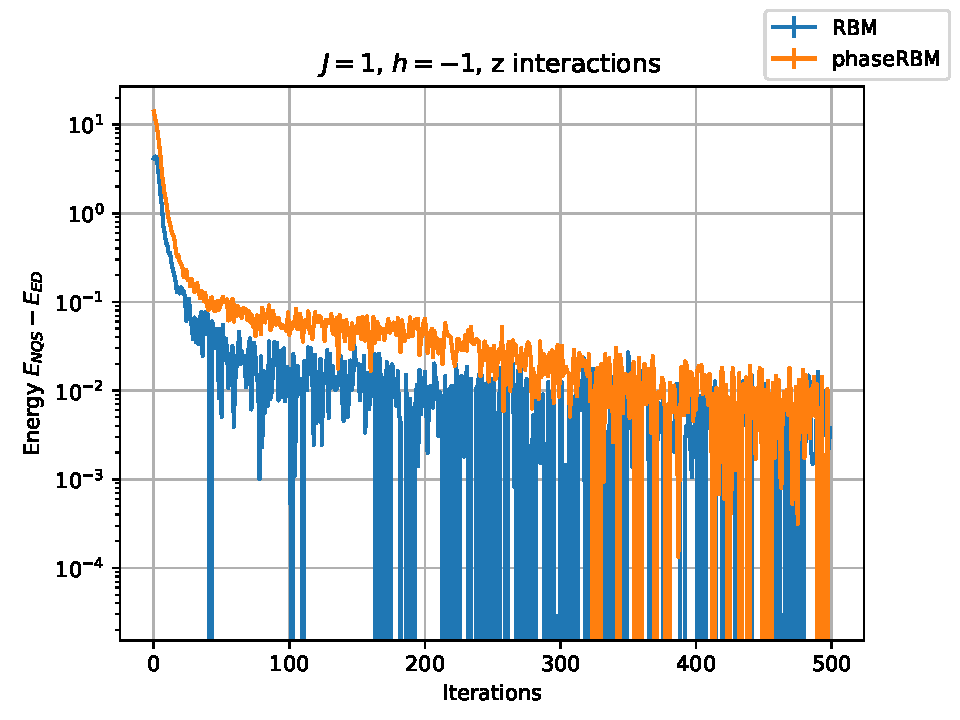
\includegraphics[height=.6\textheight]{rbm-phaserbm-comparison-log-+-.pdf}
    \end{figure}
  }
  \only<2>{
    \begin{figure}
      \centering
      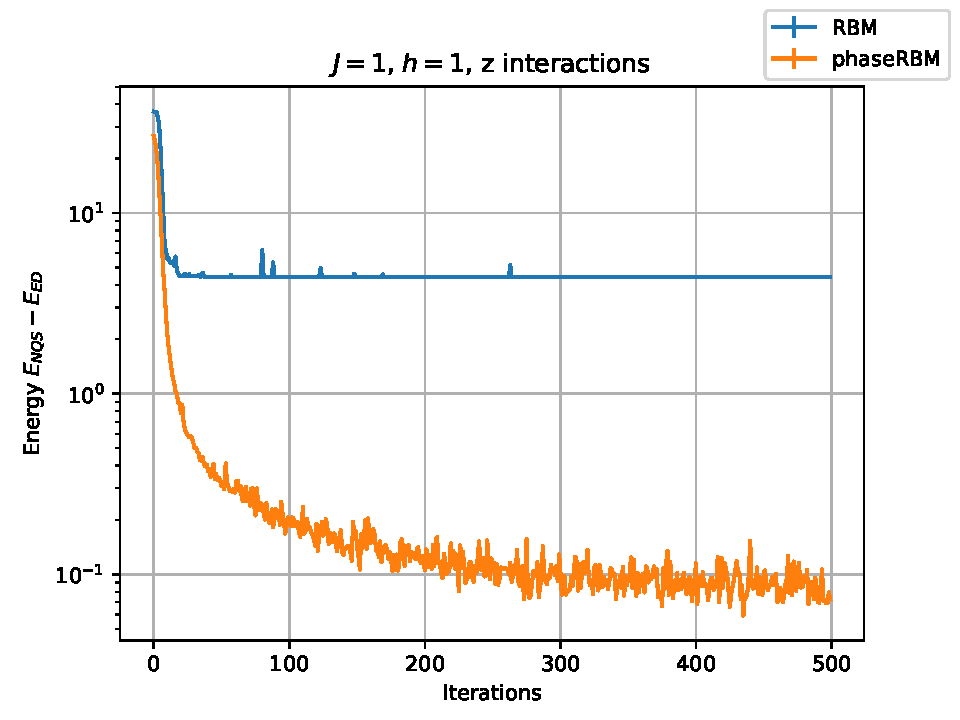
\includegraphics[height=.6\textheight]{rbm-phaserbm-comparison-log-++.pdf}
    \end{figure}
  }
\end{frame}

\begin{frame}
  \begin{figure}[h]
  \end{figure}
\end{frame}

\begin{frame}[fragile]
  \centering
  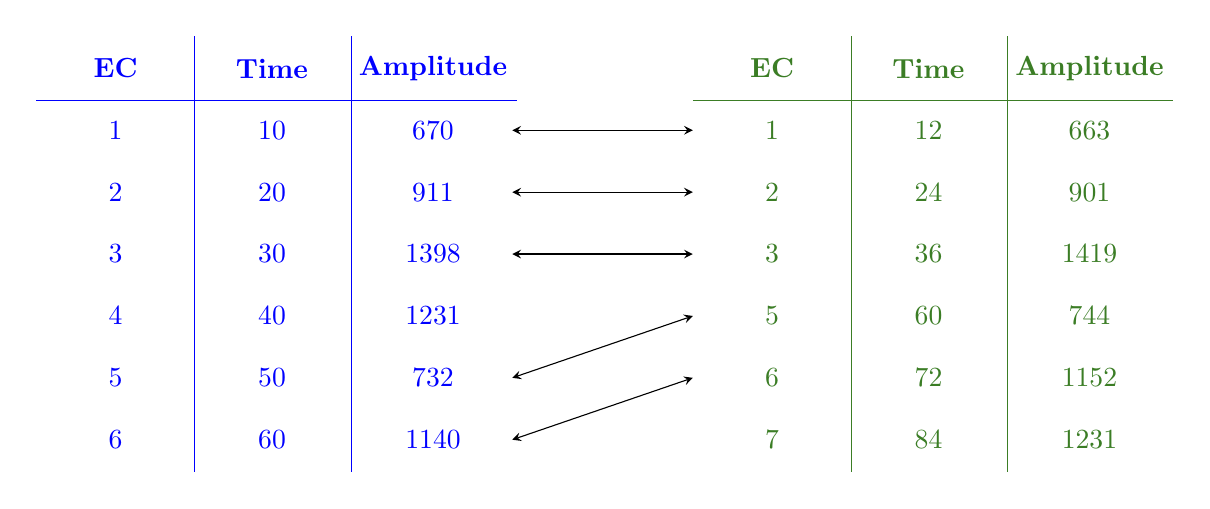
\begin{tikzpicture}[
  table/.style={
    matrix of nodes,
    nodes={minimum width=2cm, minimum height=0.8cm, anchor=center},
    column sep=-\pgflinewidth, row sep=-\pgflinewidth,
    nodes in empty cells,
  }
]

% Left table
\matrix (left) [table,text=blue] {
  \textbf{EC} & \textbf{Time} & \textbf{Amplitude} \\
  1 & 10 & 670 \\
  2 & 20 & 911 \\
  3 & 30 & 1398 \\
  4 & 40 & 1231 \\
  5 & 50 & 732 \\
  6 & 60 & 1140 \\
};

% Draw vertical separator + outer box for left
\draw[draw=blue] (left-1-1.south west) -- (left-1-3.south east);
\draw[draw=blue] (left-1-1.north east) -- (left-7-1.south east);
\draw[draw=blue] (left-1-2.north east) -- (left-7-2.south east);

% Right table
\matrix (right) [table,text=OliveGreen, right=2cm of left] {
  \textbf{EC} & \textbf{Time} & \textbf{Amplitude} \\
  1 & 12 & 663 \\
  2 & 24 & 901 \\
  3 & 36 & 1419 \\
  5 & 60 & 744 \\
  6 & 72 & 1152 \\
  7 & 84 & 1231 \\
};

% Draw vertical separator + outer box for right
\draw[draw=OliveGreen] (right-1-1.south west) -- (right-1-3.south east);
\draw[draw=OliveGreen] (right-1-1.north east) -- (right-7-1.south east);
\draw[draw=OliveGreen] (right-1-2.north east) -- (right-7-2.south east);

% Arrows between rows (automatic row anchors!)
% \draw[->] (left-2-2.east) -- (right-2-1.west);
% \draw[->] (left-3-2.east) -- (right-3-1.west);
\onslide<2>{
  \foreach \i in {2,3,4} { % horizontal rules
    \draw[<->] (left-\i-3.east) -- (right-\i-1.west);
  }
  \draw[<->] (left-6-3.east) -- (right-5-1.west);
  \draw[<->] (left-7-3.east) -- (right-6-1.west);
}

\end{tikzpicture}
\end{frame}

\begin{frame}
  \frametitle{Contents}
  \tableofcontents
\end{frame}

\section{Detection of Particles}
\begin{frame}
  \frametitle{MicroMegas Detectors}
  \begin{minipage}{.36\textwidth}
    \only<1>{
      \begin{itemize}
        \item Incoming particle ionizes gas
        \item Electrons drift to mesh
        \item Avalanche effect
        \item Signal induced in readout strips 
      \end{itemize}
      \vfill
    }
    \only<2>{
      Multiple strips for multi-channel readout
      \begin{itemize}
        % \item Number of readout channels $=$ number of strips
        \item Two orthogonal layers of strips \rarr\ 2D position information 
      \end{itemize}
      \vfill
    }
    %  \nnote{better picture (e.g. no numbers)}
  \end{minipage}
  \begin{minipage}{.62\textwidth}
    % \begin{figure}
    %   \centering
    %   \includegraphics[width=\textwidth]{micromegas-principle}
    %   \caption{\cite{wiki:micromegas-principle}}
    % \end{figure}

\centering
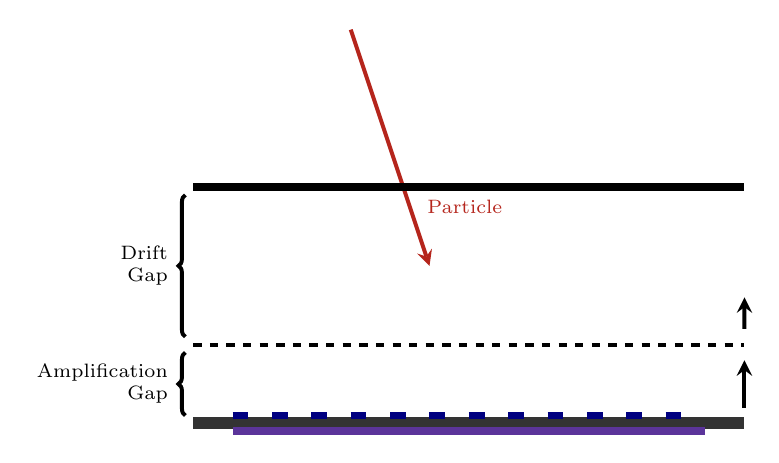
\begin{tikzpicture}[
  every node/.style={font=\scriptsize}
]
  \draw [->,draw=BrickRed,line width=.5mm] (2,5) -- (3,2) coordinate[pos=.75] (particle-arrow) coordinate[pos=1] (particle-pos);
  \node[right=1mm of particle-arrow,text=BrickRed] {Particle};
  % \node[circle,below=.5mm of particle-pos,draw=black,minimum size=.5mm] {-};

  \draw [line width=1mm] (0,3) -- (7,3) coordinate[pos=1] (cathode) coordinate[pos=0] (cathode0);
  \draw [dashed,line width=.5mm] (0,1) -- (7,1) coordinate[pos=1] (mesh) coordinate[pos=0] (mesh0);
  \draw [draw=black!80!white,line width=1.5mm] (0,0) -- (7,0) coordinate[pos=1] (anode) coordinate[pos=0] (anode0);

  \draw [->,line width=.5mm] ($(mesh) + (0,0.2)$) -- ($(mesh)!0.3!(cathode)$);
  \draw [->,line width=.5mm] ($(anode) + (0,0.2)$) -- ($(mesh) - (0,0.2)$);
  \foreach \i in {1,2,3,4,5,6,7,8,9,10,11,12} { % horizontal rules
    \draw[line width=1mm,draw=NavyBlue] ($(anode0) + \i*(0.5,0) + (0,0.1)$) -- ($(anode0) + \i*(0.5,0) + (0.2,0.1)$);
  }
  \draw[line width=1mm,draw=RoyalPurple] ($(anode0) + (0.5,0) - (0,0.1)$) -- ($(anode) - (0.5,0) - (0,0.1)$);

  \draw [decorate,decoration={brace,mirror},line width=.5mm] ($(cathode0)+(-0.1,-0.1)$) -- ($(mesh0)+(-0.1,0.1)$) coordinate[midway] (driftgap);
  \draw [decorate,decoration={brace,mirror},line width=.5mm] ($(mesh0)+(-0.1,-0.1)$) -- ($(anode0)+(-0.1,0.1)$) coordinate[midway] (ampgap);
  \node[left=1mm of driftgap,align=right] {Drift\\Gap};
  \node[left=1mm of ampgap,align=right] {Amplification\\Gap};

\end{tikzpicture}

  \end{minipage}
\end{frame}



\end{document}
